\chapter{分布式原位聚类算法系统实现}

\section{概述}
随着数据规模的快速增长,数据集中式存储的弊端越来越明显,分布式数据存储称为了常用的数据存储方式。在分布式场景下,涉及全局数据的计算则需要把各个节点数据通过网络传输到单个节点,然后再进行计算;然而很多隐私数据或涉密数据直接在网络中传输是非常危险的,可能导致机密数据的泄露或用户隐私的泄露问题,这无疑会对很多大数据公司、国家和广大用户造成巨大的损失。聚类算法,是非常依赖全局数据进行计算的,考虑数据隐私性的分布式聚类算法是目前亟待解决的问题。本系统设计背景是实验室原位计算平台,该平台则是围绕上述涉及到的问题提出一种系统解决方案,平台上聚类任务的实现则是采用了本文第三章和第四章所提出的算法。本系统开发主要利用 Java+ZooKeeper+Apache 以及 Mysql 完成,其中,前端可视化主 要利用 JavaScript+Bootstrap 进行开发,系统运行环境主要为 Ubuntu14.04 ,系统设计框架如图\ref{ch5frame}所示。
\begin{figure}[h]
	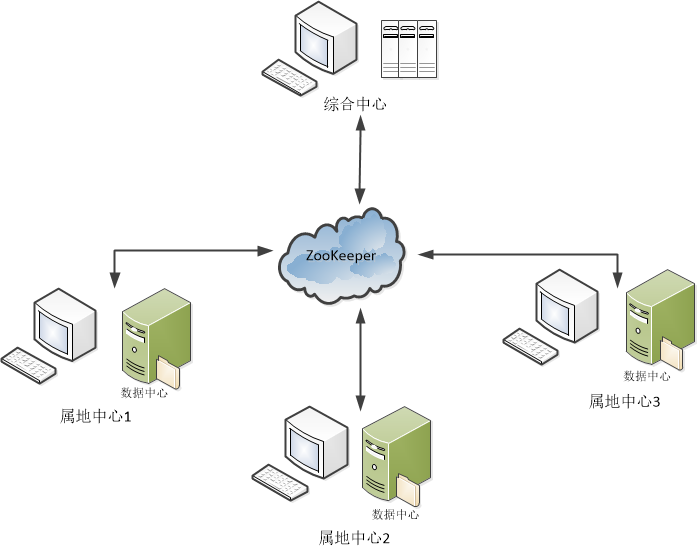
\includegraphics[height=4.5cm,width=7.5cm]{ch5frame.png}
	\caption{系统架构设计图}
	\label{ch5frame}
\end{figure}

\section{总体设计}
原位计算平台旨在为分布式各类计算任务提供解决方案,轨迹聚类计算是此平台中重点攻克的计算任务之一。本节提出了原位计算平台中轨迹聚类计算部分所涉及到的模块,主要由五个模块组成:模型训练模块、网络通信模块、综合计算模块、聚类评估模块和可视化展示模块。各模块层级结构如图\ref{ch5module}所示。
\begin{figure}[h]
	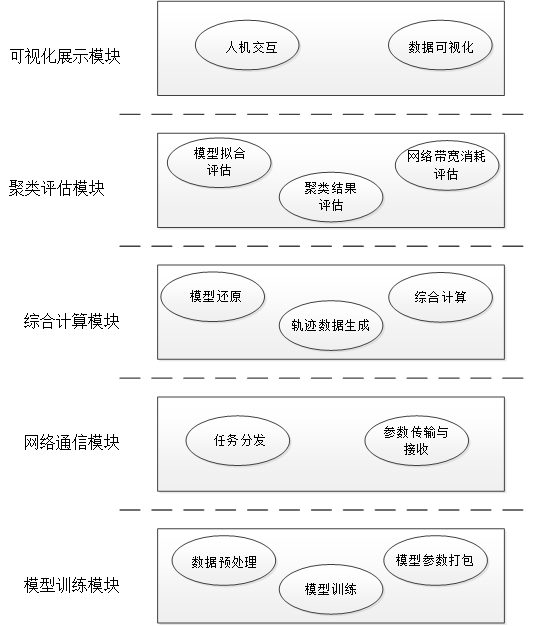
\includegraphics[height=4.5cm,width=7.5cm]{ch5module.png}
	\caption{总体模块结构图}
	\label{ch5module}
\end{figure}

现对各个模块的功能作简要阐述:
\begin{enumerate}
    \item  模型训练模块\\该模块主要负责各属地中心的局部模型训练,模块由三个部分组成:数据预处理、模型训练和模型参数打包。数据预处理部分负责将属地中心原始数据进行加工处理,使得加工后的数据能够直接用于模型训练;模型训练部分则利用数据预处理产生的数据进行轨迹生成模型估计;模型参数打包部分则是将模型训练得到的模型参数结构化,便于综合中心对于模型参数的处理。
    \item  网络通信模块\\该模块主要负责综合中心与各个属地中心的网络交互,模块由两个部分构成:任务分发和参数的传递与接收。任务分发部分负责将综合中心需要执行的计算任务分发至各个属地中心;参数的传递与接收部分主要负责综合中心和属地中心之间的信息传递以及信息同步操作。
    \item  综合计算模块\\该模块主要负责综合中心对全局数据的计算处理,模块由三个部分组成:模型还原、数据生成和综合计算。模型拟合评估是属地中心对局部生成模型拟合准确度的评估;模型还原部分是将打包好的局部模型参数还原出属地中心训练得到的轨迹生成模型;数据生成部分则通过还原的轨迹生成模型产生轨迹数据,以此来近似属地中心的轨迹数据;综合计算部分将生成的全局轨迹数据输入到聚类模型完成此次聚类计算任务。
    \item  系统评估模块\\该模块主要负责对聚类计算任务结果进行评估,模块由三部分组成:模型拟合评估、聚类结果评估和带宽消耗。模型拟合部分聚类结果评估度部分对综合计算得到的聚类结果进行评估;带宽消耗部分对此次聚类计算任务中造成的网络带宽消耗做出评价。
    \item  可视化展示模块\\该模块主要是通过可视化的界面对综合中心和属地中心的状态进行呈现,对整个系统的运行情况起到监察和管理作用。
\end{enumerate}

\section{详细设计}

\subsection{模型训练模块}
模型训练模块是属地中心利用本地轨迹数据训练轨迹生成模型的模块,其中模型的选择十分重要,对算法的准确度、带宽消耗和数据隐私性都有着至关重要的影响。第三章基于复合采样的分布式轨迹聚类算法选择了多项式拟合技术来生成轨迹数据,第四章基于马尔科夫链的分布式轨迹聚类算法选择了随机游走模型来生成轨迹数据。前者在轨迹数据还原程度上更加准确,但由于需要对每一条轨迹建模,所以带宽消耗比较大;后者在轨迹数据还原程度上没前者精确,但可以很好还原轨迹数据分布情况,而且在带宽消耗上也得到了缓解。

第三章模型训练模块流程如图\ref{ch3module}所示:
\begin{figure}[h]
	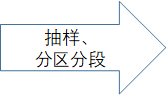
\includegraphics[height=4.5cm,width=7.5cm]{ch3module.png}
	\caption{CSD-Clustering 模型训练模块流程}
	\label{ch3module}
\end{figure}

在第三章算法中,属地中心首先对属地轨迹数据集进行了数据预处理,预处理包括轨迹数据抽样、轨迹点数抽样、分区和分段操作,然后针对每个分段轨迹构造多项式模型,利用最优化理论求解出模型参数,将模型参数格式化后形成模型参数包,模型参数包将接着由网络通信模块进行处理。

第四章模型训练模块流程如图\ref{ch4module}所示:
\begin{figure}[h]
	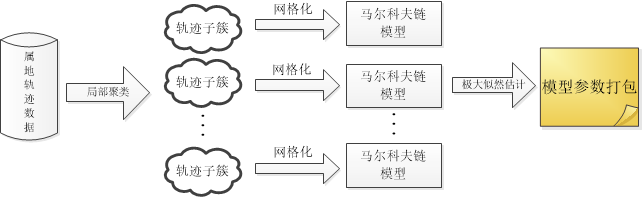
\includegraphics[height=4.5cm,width=7.5cm]{ch4module.png}
	\caption{MCD-Clustering 模型训练模块流程}
	\label{ch4module}
\end{figure}

在第四章算法中,属地中心首先对属地轨迹数据进行局部聚类处理,经过局部聚类处理后将得到若干个轨迹子簇,依据轨迹间距离度量,在各个轨迹子簇中的轨迹在轨迹走势上具有很大程度上的相似性,然后对所有轨迹进行网格化处理,使轨迹中的所有点都由网格中的点构成,对于每个网格化活动 轨迹子簇数据,构造一个马尔科夫链模型,并通过极大似然估计出概率转移矩阵中的所有转移概率,将求解出来的转移概率参数和网格化轨迹信息格式化后打包成模型参数包,模型参数包将接着由网络通信模块进行处理。

\subsection{网络通信模块}

网络通信模块提供了综合中心和属地中心在分布式环境中的相互通信功能。网络通信模块功能主要是通过ZooKeeper框架实现的,综合中心通过ZooKeeper的配置文件配置所有其他属地节点的ip地址,所有属地节点则在ZooKeeper中配置综合中心的ip地址。基于ZooKeeper实现的网络通信模块主要实现综合中心的任务分发以及所有节点(包括综合节点)的参数发送和接受,其流程如图\ref{comm}所示。
\begin{figure}[h]
\subfigure[]{
\label{centerComm}
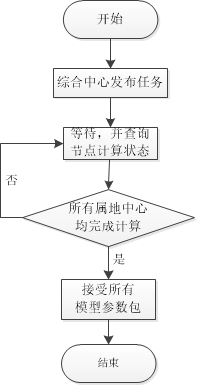
\includegraphics[height=4.5cm,width=4.5cm]{centerComm.png}
\caption{综合中心网络通信流程图}}
\subfigure[]{
\label{nodeComm}
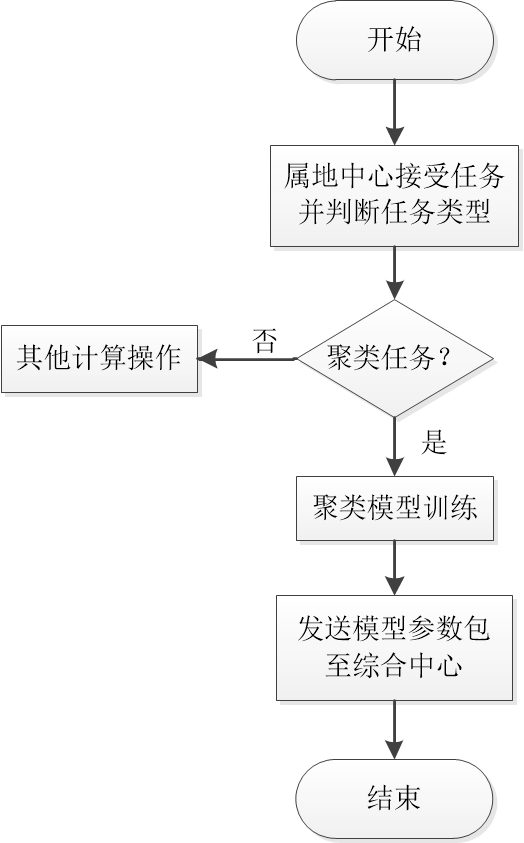
\includegraphics[height=4.5cm,width=4.5cm]{nodeComm.png}
\caption{属地中心网络通信流程图}}
\caption{网络通信流程图}
\label{comm}
\end{figure}

当综合中心发放任务时,会通过ZooKeeper向分布式环境中的所有属地中心发送计算任务信息,对于此任务,综合中心会进入等待状态,并周期性地查看计算状态,直至发现所有属地中心的计算结果均已返回,则会一次性读取所有返回的模型参数包,并进行接下来的综合计算。属地中心接收到综合中心发放的任务,首先解析任务类型,然后依据任务类型执行不同的计算操作,计算完成后将计算得到的模型参数包发送至综合中心。

\subsection{综合计算模块}

综合计算模块输入为网络通信模块传递过来的模型参数包,输出为全局聚类结果。此模块主要包含模型还原、轨迹数据生成和综合计算三个部分,若局部模型使用的模型不同,这三个部分的操作都将会不同。图\ref{compComp}展示了分别选择CSD-Clustering算法和MCD-Clustering算法所对应的综合计算流程。
\begin{figure}[h]
	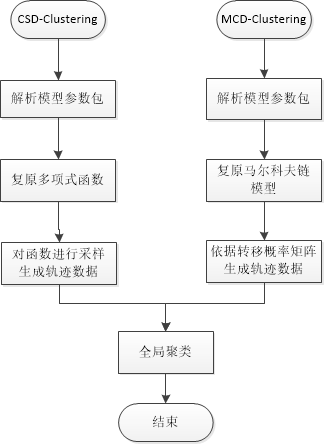
\includegraphics[height=4.5cm,width=7.5cm]{compComp.png}
	\caption{综合计算模块流程图}
	\label{compComp}
\end{figure}

对于CSD-Clustering算法对应的综合计算流程,首先从模型参数包中解析出多项式模型的系数参数,从而恢复多项式函数模型,然后从该函数模型上进行等间距采样,将采样得到的坐标点作为轨迹数据;对于MCD-Clustering算法对应的综合计算流程,首先从模型参数中解析出概率转移矩阵和初始状态,然后依据马尔科夫链产生数据的方式生成状态序列,状态序列可以转换为估计及坐标序列;得到生成的全局轨迹数据后,把轨迹数据作为输入数据输入到聚类模型中,在CSD-Clustering算法中生成的轨迹数据长度是相同的,故可以采用欧氏距离定义的k-means算法进行全局聚类操作,在MCD-Clustering算法中生成的轨迹数据长度不等,采用基于霍夫曼距离的k-medoids算法进行全局聚类操作,产生的聚类结果会输入到系统评估模块进行性能评估。

\subsection{系统评估模块}

系统评估模块故能是对此次聚类任务完成质量评估,该模块从三个方面对任务完成质量进行评估,如图\ref{evaluation}所示,分别为:局部模型拟合评估、全局聚类评估和带宽消耗。

局部模型拟合评估对于不用的局部模型评价方式也不同,对于CSD-Clustering算法,可以直接通过损失函数来刻画;对于MCD-Clustering算法,可以通过原始子簇轨迹集合和生成子簇轨迹集合之间的霍夫曼距离来刻画。全局聚类评估是对此次聚类任务结果进行评价,由于综合中心也不知道真实轨迹数据,所以只能采用内部指标对聚类本身进行评价,该系统采用DBI指数对聚类结果进行评价。带宽消耗是对本次聚类任务产生的网络通信流量情况进行展示,并原始轨迹数据统计信息可以计算出信息压缩比,体现本文提出的算法在带宽消耗上的改进。
\begin{figure}[h]
	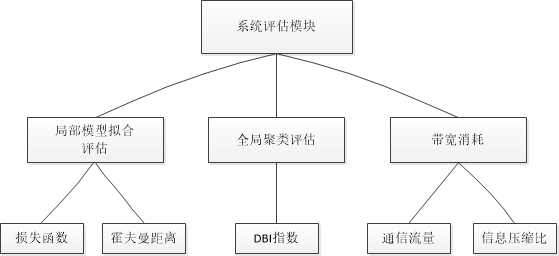
\includegraphics[height=4.5cm,width=7.5cm]{evaluation.png}
	\caption{系统评估模块}
	\label{evaluation}
\end{figure}


\section{仿真平台展示}


\section{本章小结}